\chapter{Introduction}\label{ch:introduction}

Audio interactions are becoming ubiquitous in common media platforms, consumer hardware and immersive technology \cite{yang2019audio}.

Virtual Environments (VEs), have received growing attention in the past decades \citep{rubio2017immersive}, due to their ability to reproduce real worlds in digital systems. Their applications range from computer games, including serious and educational games, to digital museums, cultural preservation and architectural design. Such applications have raised the need to realistic and compelling representations of VEs, which is achieved by emulating the physics of the real world. Performance of tasks, such as interacting with scene objects and navigating space, depends on audio-visual displays \citep{zimmons2003influence, lokki2005navigation}. Sound cues alone are sufficient to enable users in VEs to pinpoint locations of sound-emitting entities in a scene by using auditory sound localisation, a natural ability associated with the human auditory system. \par
Creating compelling and realistic auditory displays is problematic, providing many challenges in the acoustics and computer graphics research communities due to the complex nature of sound in the real world. As the acoustic principles that govern how sound propagates in space are difficult to reproduce in digital systems, many methods exist, providing variable orders of approximations, depending on the application. Such approaches emulate the wavefield of an environment, simulating how sound interacts with boundaries and scene objects. A subset of these can reproduce phenomena of sound, such as diffraction, reflection and refraction, which are determinants of realism as they emulate how waves bend around obstacles. Such phenomena make the simulated wavefield dependent on the accuracy of scene geometry and materials represented in a VE \citep{kuttruff2016room}. \par
Graphics and visual rendering systems are responsible for representing geometry and objects of an environment, defining a relationship between the appearance of materials and the simulated wavefield. This relationship determines realism and presence evoked due to the subjective aspect of auditory and visual perception.
Representation of auditory and visual information varies depending on the human sensory system. The perception of geometry and material in a complex scene is subjective, requiring rendering methods to consider aspects of human perception. 

% intro to audio rendering
Auditory information is paramount to human perception in natural and virtual environments, helping in orientation and navigation, increasing immersion and aiding in task performance \citep{lokki2005navigation, bork2015auditory, shivappa2016efficient}. The sound field perceived by a listener is a function of the shape, dimensions, boundaries and transmission mediums of the surrounding environment. Even though the physics of sound propagation makes realistic audio rendering a challenging task, many proposed approaches allow realistic simulations of sound fields in virtual environments (VEs). Computer games, compelling simulations and digital tourism benefit from realistic audio rendering and improved auditory presence evoked in virtual environments \cite{lokki2002creating, selmanovic2020vr, rubio2017immersive}.

The realism of digital media has increased in recent years thanks to recent advances in computer games technology \cite{rubio2017immersive}. Sound describes entities with respect to the acoustic environment they exist in. As a listener in a sound transmission, the human auditory system is aware of acoustic characteristics manifesting in auditory cues, which enable spatial hearing abilities, such as sound localisation, aiding interaction tasks with objects in the world. Intrinsic acoustic characteristics are dependent on the sound transmission's wavefield, dictated by structural properties of the environment, associated with boundaries and materials, as they interact with sound propagating to the listener's ears. Acoustic rendering methods simulate real or virtual auditory environments by deriving from sound propagation algorithms that discretise the geometrical representation of an environment to synthesise a wavefield. They render spatialised sound adopting signal processing chains to reproduce realistic sound transmission in the simulated wavefield, considering the listener's position, orientation and their physical characteristics, described by Head-Related Transfer Function (HRTF) \cite{hulusic2012acoustic}. \par

% Intro to Audio in XR
AR platforms are suited for a range of use cases within areas of training, digital tourism, or games, thanks to the enhanced interactions with the physical world surrounding the user. An AR platform is a set of technologies interfacing with the user via audio-visual and holographic displays, gesture, eye, and body tracking, and with the physical world via computer vision, scene understanding, space reconstruction, and spatial mapping techniques. This broad range of sensing technologies opens avenues for addressing tasks within research domains where users interact with entities in AR space. Accessibility, for instance, is a research domain benefitting from the development of this platform by helping users with disabilities navigate and understand their surrounding scene, leveraging the sensing data provided by the platform and performing speech recognition or scene understanding techniques \citep{mehra2020potential}.


The increasing popularity of immersive media proliferating within an increasing number of industry and research domains \citep{park2022metaverse}, enabling HMDs to support applications ranging from training scenarios, education, social learning, operation learning \citep{harris2020effect, ahir2020application} to entertainment or gaming \citep{yuen2011augmented, ke2018virtual} or to digital tourism and cultural preservation use cases \citep{schofield2018viking, selmanovic2020cultural}. AR applications in modern HMDs, e.g. the Microsoft Hololens 2\footnote{\url{https://www.microsoft.com/en-gb/hololens}\label{note:ms-hl2}}, can provide real-time space reconstruction, spatial mapping, and scene understanding features\footnote{\url{https://learn.microsoft.com/en-us/hololens/hololens2-hardware}\label{note:ms-hl2-hw}}. Such features have unlocked crucial potential in the sound rendering subdomain, as emerging novel pipelines allow acoustic simulation techniques to be deployed to AR HMDs, as discussed in Chapter~\ref{ch:ar-pipeline}. As a result, users experiencing holographic content projected onto their surroundings can perceive realistic sound propagation from holograms. Experiencing realistic sound rendering in AR directly impacts the above-mentioned industry domains and research as HMDs become more ubiquitous and accessible. \par
These example applications and use cases of AR with modern HMDs rely on auditory stimuli for conducting activities or completing tasks in VEs, such as navigation, locomotion, or entity localisation. As discussed in Chapter~\ref{ch:Background}, the hearing sense relies on acoustic information encoded in auditory stimuli to predict or triangulate the position of sound-emitting objects within the hearing range.


\section{Significance}
A novel aspect of the proposed work is the application of computer vision methods to infer acoustic data associated with materials and boundaries in environments to enable sound rendering systems such as acoustic simulation methods, to adapt to unseen complex scenes in materials.
Potential contributions of this novelty include Augmented Reality (AR) applications \citep{liu2018technical}, where users can control interactions between virtual objects and the real world. A possible outcome from the proposed work would allow AR applications to render sounds emitted from virtual objects considering acoustic aspects of real environments. \par
The system would apply to computer games technology, contributing to computer games, serious games, architectural acoustics and digital tourism. 
Architectural acoustic applications would benefit from automated reconstructions of auditory spaces from real environments, allowing designers to create and test acoustic models with AR applications or game engines \citep{berardi2016acoustic}. Digital tourism, besides, would benefit from improvements in sound rendering pipelines to let users experience and interact with reconstructions of places of cultural interest \citep{schofield2018viking}. \par
The need for realistic audio in computer games is of growing importance as it allows players to immerse in virtual worlds. Spatialising sound in three-dimensional worlds, reflecting acoustic features of space, improves the performance of tasks associated with auditory cues, enhancing the overall experience and quality in games. 
Activities in VEs using auditory cues, such as navigation in space and sound localisation are fundamental in simulations and training applications \citep{lokki2005navigation}. Hence, sound rendering systems are of crucial importance in these fields.

\section{Research Aim}
\begin{figure}[htbp]
    \centering
    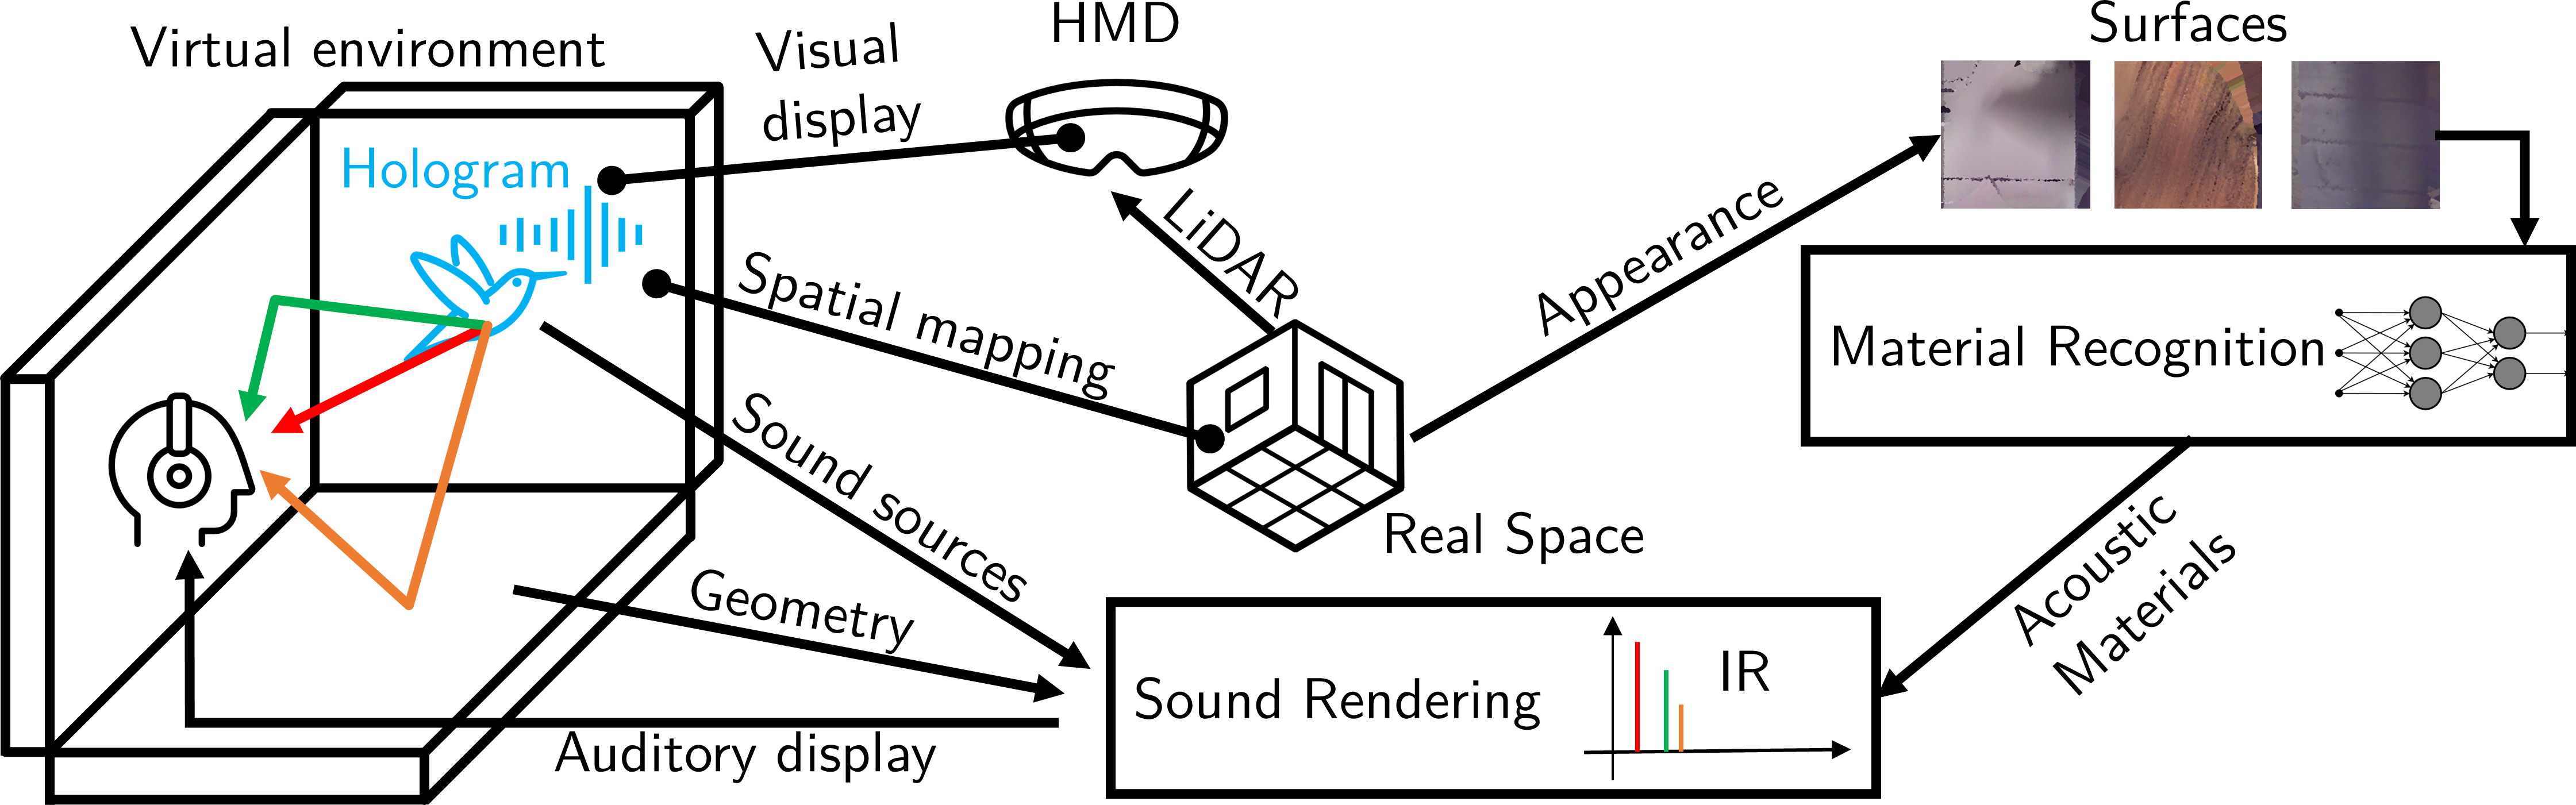
\includegraphics[width=1\linewidth]{phd_functional_diagram}
    \caption{Overview of the interactive acoustic rendering system for AR proposed as part of the thesis work.}
    \label{fig:proposed-system-diagram}
\end{figure}
The proposed work aims to explore rendering pipelines with respect to sound propagation in VEs, studying the relationship between the perceived wavefield and the environment’s visual representation: materials, structural geometry and physicals characteristics of objects in complex scenes.


\section{Objectives}\label{sec:thesis-objectives}
\begin{itemize}
    \item To review the current state of audio rendering in virtual environments, assessing their limitations, realism and computational requirements to  investigate their applications in real-time acoustic simulations for complex scenes.
    \item To explore how, in modern approaches to acoustic simulations, visual representations of materials relate to simulated soundfields.
    \item To design and test systems to automatically attribute acoustic materials to scene geometry in virtual environments, recognising and distinguishing between materials in the acoustic and visual domains.
    \item To study and evaluate the application of sound rendering methods with acoustic material recognition.
    \item To design and propose a novel pipeline for acoustic rendering applied to augmented reality platforms.
    \item To investigate psychoacoustic and human factors in auditory displays created by the proposed pipeline by testing an augmented reality prototype.
\end{itemize}

\section{Thesis Structure}

\begin{figure}[htbp]
    \centering
    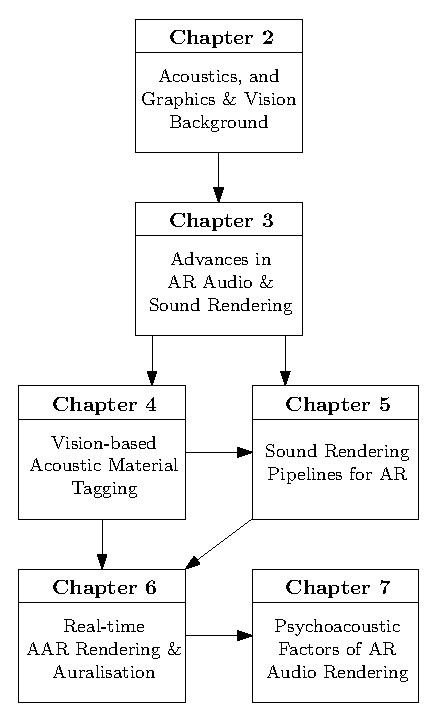
\includegraphics[width=0.6\linewidth]{thesis-structure}
    \caption{Structure and dependency graph of Chapters of this thesis. Introductory and conclusive Chapters, \ref{ch:introduction} and \ref{ch:Conclusion} respectively, omitted for simplicity.}
    \label{fig:thesis-structure}
\end{figure}

\section{Chapter List}
\textbf{Chapter \ref{ch:introduction}} Introduction presents the goal and objectives to the reader, starting from the rationale and factors motivating this research, providing background on research domains of interest, and illustrating the contributions and how these are structured throughout the Chapters.

\textbf{Chapter \ref{ch:Background}} Background Research provides the reader with foundations on wave physics, sound propagation, acoustic data in digital systems, as well as computer graphics in the context of handling and representing virtual environments. The reader is also introduced to elements of machine learning to provide grounding for vision-based scene understanding systems designed as part of the thesis aim.

\textbf{Chapter \ref{ch:litReview}} Advances in Visual-Acoustic Mapping Methods and Sound Rendering Pipelines reports relevant bodies of literature relevant to research and industry domains overlapped by the proposed overarching system. Limitations of the current state of industry and research on these domains are reviewed alongside visions and research directions identified by authors, defining the contributions discussed across the thesis.

\textbf{Chapter \ref{ch:Materials}} Methods for Acoustic Characteristics Retrieval from Complex Virtual Environments introduces the design and application of computer vision methods for extracting acoustic characteristics from virtual environments, which constitute building blocks for the proposed pipeline and address acoustic material tagging, a crucial problem in the domain of sound propagation for virtual environments.

\textbf{Chapter \ref{ch:acousticrendering}} Geometrical Acoustics Rendering Pipelines for Augmented Acoustics integrates acoustic material tagging systems with standard acoustic rendering techniques based on approximating acoustic waves with geometrical primitives. This Chapter aims to provide a baseline acoustic renderer for designing the interactive AR pipeline proposed in the following Chapter.

\textbf{Chapter \ref{ch:ar-pipeline}} Towards Scene-Aware Acoustic Rendering Pipelines for Augmented Audio Reality demonstrates the design of the proposed pipeline, expressed by the overarching research aim, as an end-to-end system for Augmented Reality Head-Mounted Displays, illustrating technical components and workflows for achieving real-time interactions. Considering related work reviewed by Chapter\ref{ch:litReview}, visions, impact and future research are discussed, indicating avenues for expansions.

\textbf{Chapter \ref{ch:Conclusion}} Conclusions provides a high-level discussion on the results gathered from objective and subjective experiments gathered by testing components of the proposed system, reflecting on broader impact, detailing potential use cases, and recommending future expansion avenues.

\section{Contributions}
The main contributions of this thesis are the proposal, design, prototyping, and testing of a novel pipeline for generating realistic auditory displays in augmented reality platforms, leveraging the potential that modern hardware for holographic rendering has unveiled over the last decades. These contributions represent a stepping stone towards realistic and physically-based auditory interactions in immersive applications, allowing users to understand, reason, and act within a virtual environment from acoustic information conveyed by the augmented reality platform.
These contributions stem from components of the pipeline developed and tested, addressing research questions associated with the design of an end-to-end system. Chapters~\ref{ch:Materials},~\ref{ch:acousticrendering}, and~\ref{ch:Evaluation} present novel systems to address such research questions adopting bespoke methodologies and evaluations. The following list briefly summarises the contributions of this work:
\begin{itemize}
    \item a novel pipeline for realistic acoustic displays for augmented reality platforms;
    \item two novel systems for retrieving acoustic characteristics from virtual environments;
    \item novel testing methodologies for evaluating system for acoustic characteristics retrieval, comparing simulated against real soundfields;
    \item two sound rendering systems integrating methods for acoustic characteristics retrieval;
    \item a study evaluating the proposed sound rendering methods;
    \item a perceptual evaluation investigating psychoacoustic factors of a prototype of the proposed system.
\end{itemize}

% \fullcite{colombo2021texture}